%% FEUP THESIS STYLE for LaTeX2e
%% how to use feupteses for MIEIC dissertations
%%
%% FEUP, JCL & JCF,  Wed Oct  4 16:32:24 2017
%%
%% PLEASE send improvements to jlopes at fe.up.pt and to jcf at fe.up.pt
%%

%%========================================
%% Commands: pdflatex pdis
%%           bibtex pdis
%%           makeindex pdis (only if creating an index) 
%%           pdflatex pdis
%% Alternative:
%%          latexmk -pdf pdis.tex
%%========================================

\documentclass[11pt,a4paper,twoside,openright]{report}
\usepackage[utf8]{inputenc}
\usepackage{rotating}
%\usepackage[latin1]{inputenc}

%%%%%%% English version 

%% MIEIC options
\usepackage[mieic]{feupteses}                  % work version
%\usepackage[mieic,juri]{feupteses}             % juri verrion
%\usepackage[mieic,final]{feupteses}            % final version

%% Additional options for feupteses.sty: 
%% - portugues: titles, etc in portuguese
%% - onpaper: links are not shown (for paper versions)
%% - backrefs: include back references from bibliography to citation place

%%%%%%% Portuguese version

%\usepackage[mieic,portugues]{feupteses}        % work version
%\usepackage[mieic,portugues,juri]{feupteses}   % juri version
%\\usepackage[mieic,portugues,final]{feupteses}  % final version

%% Uncomment the next lines if side by side graphics used
%\usepackage[lofdepth,lotdepth]{subfig}
%\usepackage{graphicx}
%\usepackage{float}

%% Include color package
\usepackage{color}
\definecolor{cloudwhite}{cmyk}{0,0,0,0.025}

%% Include source-code listings package
\usepackage{listings}
\lstset{ %
 language=C,                        % choose the language of the code
 basicstyle=\footnotesize\ttfamily,
 keywordstyle=\bfseries,
 numbers=left,                      % where to put the line-numbers
 numberstyle=\scriptsize\texttt,    % the size of the fonts that are used for the line-numbers
 stepnumber=1,                      % the step between two line-numbers. If it's 1 each line will be numbered
 numbersep=8pt,                     % how far the line-numbers are from the code
 frame=tb,
 float=htb,
 aboveskip=8mm,
 belowskip=4mm,
 backgroundcolor=\color{cloudwhite},
 showspaces=false,                  % show spaces adding particular underscores
 showstringspaces=false,            % underline spaces within strings
 showtabs=false,                    % show tabs within strings adding particular underscores
 tabsize=2,	                    % sets default tabsize to 2 spaces
 captionpos=b,                      % sets the caption-position to bottom
 breaklines=true,                   % sets automatic line breaking
 breakatwhitespace=false,           % sets if automatic breaks should only happen at whitespace
 escapeinside={\%*}{*)},            % if you want to add a comment within your code
 morekeywords={*,var,template,new}  % if you want to add more keywords to the set
}

%% Uncomment to create an index (at the end of the document)
%\makeindex

%% Path to the figures directory
%% TIP: use folder ``figures'' to keep all your figures
\graphicspath{{figures/}}

%%----------------------------------------
%% TIP: if you want to define more macros, use an external file to keep them
%some macro definitions

% format
\newcommand{\class}[1]{{\normalfont\slshape #1\/}}

% entities
\newcommand{\Feup}{Faculdade de Engenharia da Universidade do Porto}

\newcommand{\svg}{\class{SVG}}
\newcommand{\scada}{\class{SCADA}}
\newcommand{\scadadms}{\class{SCADA/DMS}}

%%----------------------------------------

%%========================================
%% Start of document
%%========================================
\begin{document}

%%----------------------------------------
%% Information about the work
%%----------------------------------------
\title{Automatic C/C++ source-code normalization and optimization}
\author{João Nuno Matos}

%% Uncomment next line for date of submission
%\pdisdate{July 31, 2008}

%%Uncomment next line for copyright text if used
%\copyrightnotice{Name of the Author, 2008}

\supervisor{Supervisor}{João Bispo}

%% Uncomment next line if necessary
%\supervisor{Second Supervisor}{Name of the Supervisor}

%% Uncomment committee stuff in the final version 
%\committeetext{Approved in oral examination by the committee:}
%\committeemember{Chair}{Doctor Name of the President}
%\committeemember{External Examiner}{Doctor Name of the Examiner}
%\committeemember{Supervisor}{Doctor Name of the Supervisor}

%\committeetext{Aprovado em provas públicas pelo Júri:}
%\committeemember{Presidente}{Nome do presidente do júri}
%\committeemember{Arguente}{Nome do arguente do júri}
%\committeemember{Vogal}{Nome do vogal do júri}

%% Uncomment signature line in the final on paper version
%\signature

%% Specify cover logo (in folder ``figures'')
\logo{uporto-feup.pdf}

%% Uncomment next line for additional text below the author's name (front page)
\additionalfronttext{Preparação da Dissertação}

%%----------------------------------------
%% Preliminary materials
%%----------------------------------------

% remove unnecssary \include{} commands
\begin{Prolog}
  \chapter*{Abstract}

Modern compiled software, written in languages such as C and C++, relies on complex compiler infrastructure that transforms programs in ways that improve their non-functional characteristics. However, developing new transformations and improving existing ones can be challenging to researchers and engineers. Often, transformations are conceived in terms of the high-level language, but must be implemented by transforming a lower-level intermediate representation (IR) or by modifying the compiler itself, which may not be feasible, for technical or legal reasons.

Source-to-source compilers make it possible to directly analyze and transform the original source, making transformations portable across different compilers. This approach allows transformations to be composed upstream of the compilation toolchain, allowing rapid research and prototyping of source code transformations, and its use has been proposed as a solution for implementing program transformations whenever it would prove to be infeasible or impractical to do so at the compiler level. One such tool is Clava, which embeds a scriptable Javascript environment and provides access to the Abstract Syntax Trees of C and C++ programs, allowing the source code to be queried and manipulated.

However, this approach has the drawback of exposing the researcher to the full breadth of the source language, which is often more extensive and complex than the IRs used in traditional compilers. Because of that complexity, it is hard to perform complete analyses that can account for all edge cases in the language. On the other hand, those constructs, such as loops or structures, can be useful to encode properties that are not made explicit in lower-level representations.

In this work, we propose a solution to tame the complexity of the source language and make source-to-source compilers an ergonomic platform for program optimization work, by dividing the transformations into two distinct steps. First, we define a simpler subset of the language that can encode the programs with fewer primitives, and implement a set of transformations, termed normalizations, to transform the input programs into equivalent programs expressed in that subset. Afterwards, we implement a function inlining transformation as a case study, showing how the assumptions afforded by using a simpler language subset allow us to successfully apply the transformation to codes that would otherwise not be able to be transformed.

We validate our experiment and evaluate our work by comparing the application of optimizations with and without normalization, in terms of the number of transformation cases successfully applied and the performance of the resulting programs, and test the composability of several transformations. On the one hand, the inlining transformations we tested were able to take advantage of the normalized language, regardless of whether they were developed with a normalized program in mind. Our performance testing also suggests that, in general, source-to-source compilation is a good technique to apply optimizations when using less developed compilers. On the other hand, we observed challenges when composing our transformations with existing source-code transformations, which expected  primitives that were not kept in the subset, such as for loops.

\vspace*{10mm}\noindent
\textbf{Keywords}: source-to-source compilers, source-code optimization, source-code normalization

\chapter*{Resumo}

O software compilado de hoje (escrito por exemplo em C ou C++) depende de infraestruturas de compilação complexas que transformam programas de maneira a melhorar as suas caraterísticas não funcionais. No entanto, desenvolver novas transformações e melhorar as existentes pode provar-se um desafio para investigadores e engenheiros. Frequentemente, as transformações são concebidas pensando na linguagem de alto nível, mas precisam de ser implementadas como transformações de uma representação intermédia (IR) menos abstrata, ou mesmo através de modificações dos compiladores, o que poderá não ser viável por motivos técnicos ou legais.

Os compiladores \textit{source-to-source} permitem analisar e transformar diretamente o código-fonte original, tornando as transformações portáteis entre diferentes compiladores. Esta abordagem permite que as transformações sejam compostas a montante das ferramentas de compilação, permitindo uma rápida investigação e prototipagem de transformações de código, e o seu uso tem sido proposto como uma solução para a implementação de transformações de programas, sempre que fazê-lo ao nível dos compiladores seja inviável ou inconveniente. Uma dessas ferramentas é o Clava, que contém um ambiente de execução programável em Javascript e dá acesso às Árvores de Síntaxe Abstratas de programas em C e C++, permitindo a interrogação e transformação do código-fonte.

No entanto, esta abordagem tem a desvantagem de expor o investigador a toda a largura da linguagem de fonte, que frequentemente é mais extensa e complexa do que as IRs usadas nos compiladores tradicionais. Devido a essa complexidade, é difícil efetuar análises completas, que possam ter em conta todos os detalhes e exceções da linguagem. Por outro lado, estes construtos, como ciclos e estruturas, podem ser úteis para codificar propriedades que não são explícitas nas representações de nível mais baixo.

Neste trabalho, propomos uma solução para domar a complexidade da linguagem de fonte e tornar a compilação \textit{source-to-source} uma plataforma ergonómica para trabalho de otimização de programas, através da divisão das transformações aplicadas em dois passos distintos. Primeiro, definimos um subconjunto simplificado da linguagem, que possa codificar os programas escritos nela com menos primitivas, e implementamos um conjunto de transformações, apelidadas de normalizações, para transformar os programas-alvo em programas equivalentes expressos nesse subconjunto. De seguida, implementamos uma transformação de \textit{inlining} como caso de estudo, mostrando como as assunções que emergem do uso da linguagem simplificada permitem-nos aplicar com sucesso a transformação a códigos à qual esta não seria aplicável.

Validamos a nossa experiência e avaliamos o nosso trabalho, comparando a aplicação de otimizações com e sem normalização, em termos do número de casos transformáveis e do desempenho dos programas resultantes, e testamos a capacidade de composição de várias transformações. Por um lado, as transformações de \textit{inlining} testadas foram beneficiadas pelo processo de normalização, independentemente de terem sido desenvolvidas com programas normalizados em mente. Os nossos testes de desempenho também sugerem que a compilação \textit{source-to-source}, genericamente, é uma boa técnica para aplicar otimizações em conjunto com compiladores menos desenvolvidos. Por outro lado, observamos desafios ao compor as nossas transformações com transformações de código-fonte pré-existentes, que esperavam primitivas que não foram mantidas no subconjunto, tais como ciclos \textit{for}.

\vspace*{10mm}\noindent
\textbf{Keywords}: compiladores source-to-source, otimização de código fonte, normalização de código fonte
  % the abstract
  \chapter*{Acknowledgements}
%\chapter*{Agradecimentos}

Thank you,

\flushleft{My family: to my parents for fostering me to be curious and knowledgeable, and helping me explore the world over the years; to my godparents for supporting me and being the stern voice when I am too bohemian; to my brother, for making me angry, laugh, and cry with joy.}

\flushleft{My friends from Matosinhos: to Luís, Francisco, Pedro, Diogo, Gonçalo, Filipa, Tiago, Tozé, Matilde, and Martins, for sharing so many years and important milestones. To Eduardo and Leonor for putting up with me in our adventures and staying close to me no matter what.}

\flushleft{My friends from university: to Bernas, Vítor, Luís, Miguel, Cajó, Pedro, Tito, for being the best mates I could ask, right from the start. To Manel, the one that got away. To André, for being my role model and inspiration to always do better in our field.}

\flushleft{To João Macedo, for being my brother in arms. For the times we spent as teens, for the trips we made, for the miles we walked together, for the calls, for the nights out bar crawling and the nights in pulling all-nighters coding, for Berlin and Valencia, for all else we shared. You started as a drop-in from Computer Engineering, and now look where you are. I've seen you grow so much, and grown up so much myself, and I cannot shake how much of a privilege it is to have you in my life.}

\flushleft{To professor João Bispo for supervising my thesis work. For being the approachable professor in Compilers and Software Language Engineering, for being enthusiastic in the work I was doing and pushing me to consider the broader context and consequences of it. For being my editor, correcting and nitpicking and making me a better author.}

\flushleft{To David, Teté, Pedro Nuno, Carolina Losada, Bernardo Moreira, Luís Sousa, and so many others.}

\flushleft{Yours sincerely,}
\flushleft{João}
   % the acknowledgments
  \cleardoublepage
\thispagestyle{plain}

\vspace*{8cm}

\begin{flushright}
  \textsl{``Try looking into that place where you dare not look!\\
  You'll find me there, staring out at you!''}\\
\vspace*{0.8cm}
    Frank Herbert \\
    (probably writing about software bugs)
\end{flushright}
     % initial quotation if desired
  \cleardoublepage
  \pdfbookmark[0]{Table of Contents}{contents}
  \tableofcontents
  \cleardoublepage
  \pdfbookmark[0]{List of Figures}{figures}
  \listoffigures
  \cleardoublepage
  \pdfbookmark[0]{List of Tables}{tables}
  \listoftables
  \chapter*{Abbreviations}
\chaptermark{ABBREVIATIONS}
%\chapter*{Acrónimos}
%\chaptermark{ACRONIMOS}


\begin{flushleft}
\begin{tabular}{l p{0.8\linewidth}}
IR      & Intermediate Representation\\
DSL     & Domain-Specific Language\\
SSA     & Single Static Assignment\\
AST     & Abstract Syntax Tree
\end{tabular}
\end{flushleft}

  % the list of abbreviations used
\end{Prolog}

%%----------------------------------------
%% Body
%%----------------------------------------
\StartBody

%% TIP: use a separate file for each chapter
\chapter{Introduction} \label{chap:intro}

\section*{}

Modern compiled software is written in languages, such as C and C++, that allow the author to abstract themselves away from the implementation details of the machine or lower level abstractions, and focus on properly encoding the functional requirements of their application. However, to do so, we rely on modern compilation toolchains, such as LLVM and GCC, to optimize our programs and ensure they satisfy non-functional requirements such as performance and efficiency.

Moreover, developers usually expect that these transformations are applied automatically, or by supplying minimal amounts of configuration. Developers usually choose a level of optimization along a scale that balances a trade-off between compilation times and the number or complexity of performed optimizations, or, in rarer and more advanced cases, might manually enable or disable certain optimizations, or insert directives in the source-code to guide the compiler.

\section{Context} \label{sec:context}

Generally, \textit{compilers} are tools that read code, usually written in a high-level, human-readable language, and translate the code to another language, usually low-level and for machines (e.g. machine code, byte-code). Compilers can apply a number of transformations during translation, to meet certain objectives, usually on a intermediate representation (IR), that lowers the code from language-specific constructs but that abstracts away platform-dependent concepts.\cite{LattnerAOSA} \textit{Optimizing compilers} focus especially on transformations that improve the code's performance and efficiency characteristics.

These transformations can be classified as \textit{optimizations}, which directly contribute to improving the programs' performance, and/or \textit{enabling transformations}, which, irrespective of their direct performance impact, might enable or facilitate further optimizations. An example of an optimization is constant folding, which directly reduces the amount of work done at run time, and an example of an enabling transformation is function inlining, which may or may not improve performance, but has the further effect of enabling further optimizations across function boundaries.

\textit{Source-to-source compilers} are compilers whose output, instead of being low-level code, is code in the same or a different, but still high-level, human-readable language (in this case they are commonly named \textit{transpilers}). Clava is a source-to-source compiler, developed at FEUP and based on the LARA framework and Clang, that supports the use of a Javascript-based domain specific language (DSL) to transform C and C++ programs, by manipulating their Abstract Syntax Trees (ASTs).

\section{Motivation} \label{sec:motivation}

To research, prototype, and implement novel compilation techniques, the traditional approach has been for researchers to extend existing compilers and implement transformation passes on their low-level IR. This process presents a number of challenges:

\begin{enumerate}
    \item Because the compiler IRs have a lower level of abstraction, the researcher meets a higher learning curve when performing their work, because they must represent their transformation in terms of those low-level primitives instead of the semantics of the target language. Furthermore, some semantic details of the high-level language that might be useful in performing the transformation are frequently lost in translation to the low-level IR, or are only recovered after performing complex analysis of the low-level code \cite{Zangerl2018}.
    \item The low level of abstraction of the most used IRs (e.g., LLVM-IR \cite{Lattner2004}) ties the effort to a specific computing model, e.g. the von Neumann machine, even when the semantics of the transformation are applicable to a larger range of computing models, if encoded in terms of the high-level language \cite{Lattner2021}.
    \item Because each compiler tends to have its own Intermediate Representation, supporting transformations that have been encoded in terms of one IR to another compiler toolchain requires non-trivial porting and duplication of effort. This means that custom compiler passes become tied to a specific compiler.
    \item Often it is not feasible to modify the compiler. This may be a practical issue, e.g. because modifications must be either coordinated with upstream developers or a separate fork must be maintained over an extended period of time, or a regulatory issue: some projects, such as those in the automotive industry, may need to use certified compilers that need to be kept deliberately simple, or the cost of certifying those transformations is prohibitive.
\end{enumerate}

A complementary approach that has been proposed to address these issues is the use of source-to-source compilers as the first step in the compilation toolchain. By encoding the semantics of the transformation in terms of the source language, challenges 1 and 2 are adddressed, since the semantic model of the the original source code is preserved, and is not restricted to a specific target architecture. By generating as the output a program in the source language, challenges 3 and 4 are addressed, since the ability to reuse the underlying compilation infrastructure is preserved, and existing optimization work can be re-purposed.

However, this approach is not without caveats. The most important of these is that a high-level language, by design, presents an extensive set of syntactical and semantic constructs, which, by confronting the compiler developers with an increasing number of semantic primitives and an explosion of the number of interactions between them, increasingly requires more complex analyses.

To control this complexity, compiler developers have begun implementing multiple tiers of IRs, which aim to balance different levels of expressibility (higher-level abstractions) and parsimony (lower-level primitives). However, this approach of restricting the semantics of the language to a subset by \textit{construction} eschews the ease-of-use benefits of source-to-source compilation, by requiring compiler developers to work with even more models and languages.

Our work presents an alternative approach that can be taken, specifically within the context of a source-to-source compiler. We present a technique to simplify the high-level language by a process of \textit{subtraction}. This process exploits the wealth of primitives present in the high-level language, by rewriting specialized language constructs in terms of their more general counterparts. That way, we are left with a simpler program, still in the source language, that can be confidently targeted by simpler analyses and transformations.

\section{Objectives} \label{sec:objectives}

Taking into account the context and our motivation, we set out with three research questions:

\begin{enumerate}
    \item What are the techniques that are used, both traditionally and in recent developments, to manage the complexity of program representations and enable analysis and optimization work?
    \item What is the minimum subset of the C and C++ languages that allow an expressive representation of programs, while being more amenable to program analysis and transformation in a source-to-source compilation environment, such as Clava?
    \item Can an optimization be prototyped, following the normalization of programs to this subset, that produces measurable effects on their non-functional characteristics, namely performance?
\end{enumerate}

\section{Document Structure} \label{sec:struct}

In this first chapter, Chapter~\ref{chap:intro}, we discuss the context in which the work is undertaken, the motivation, and its expected objectives.
Chapters \ref{chap:sota-bg} and \ref{chap:sota-lit} discuss the state of the art that is relevant to provide context to the work. Chapter \ref{chap:sota-bg} provides the background needed to understand this work, namely discussing the architecture that compiler engineers have developed to streamline the process of supporting compilation and program transformation while simultaneously targeting multiple source languages and target platforms, and categorizing the scope and nature of code analyses and transformations. Having this background in mind, as well as the challenges to traditional approaches that were described in Chapter \ref{chap:intro}, we go over and summarise what other approaches have been taken to solve these problems, including approaches based on constructing IRs with different levels of abstraction, and earlier contributions that precede our work.
Chapter \ref{chap:gen_approach} details the general approach that we have taken to architect, implement, validate and evaluate our proposed solution.
Chapter \ref{chap:subset} describes the theoretical framework that we developed to guide our language normalization effort, and enumerates the analyses and normalization steps that we derived and implemented based on that framework.
Chapter \ref{chap:inlining} details a case study that we developed to validate our normalization approach, contributing a source-to-source function inlining transformation that is able to leverage the normalized subset to inline functions in cases where it would not be possible before.
In Chapter \ref{chap:evaluation} we present three experiments that we performed to evaluate the enabling effects of our normalization transformations and the performance and enabling effects of our inlining transformation, and discuss the results we obtained.
In Chapter \ref{chap:conclusions} we summarize our contributions and results, discuss the outcomes of our work, and reflect on the shortcomings of our contributions, proposing possible avenues to be explored in future works.
 
\chapter{Background} \label{chap:sota-bg}

\section{Architecture of Traditional Optimizing Compilers}

Fully discussing the history of compiler construction is out of scope for this work. However, we present an overview of the architecture of modern compilers, taking as examples LLVM, GCC, and CompCert.

Modern, retargetable compilers emerged to solve the so-called \textit{$m \times n$ problem}: how can we reduce the work of providing a compilation infrastructure that support a set of source languages (such as C, C++, FORTRAN, Ada, Rust, and so on) and yet also be able to generate optimized code for several hardware architectures (such as x86 and x86-64, Arm, POWER, RISC-V, and so forth), while avoiding a combinatorial explosion of implementation effort?

\begin{figure}
    \centering
    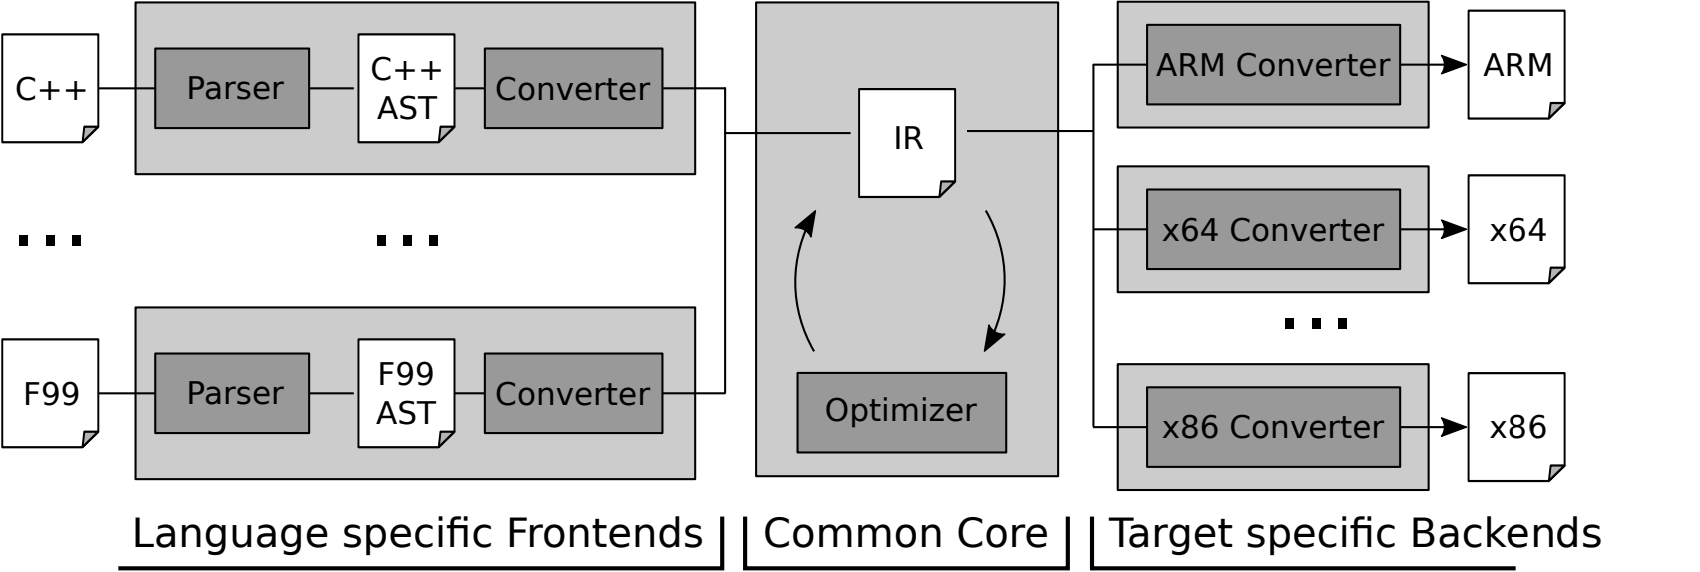
\includegraphics[width=\textwidth]{figures/generic_compiler_arch.png}
    \caption{A conceptual model of a retargetable compiler. Re-printed from \cite{Zangerl2018}}
    \label{fig:generic_compiler}
\end{figure}

To do so, they relied on two key insights: that these high-level languages were able to be transformed down to equivalent code in a subset of core imperative primitives that is still hardware-independent, and that this low-level intermediate representation (IR) contains enough information to perform most common optimizations.

Therefore, as seen in Figure~\ref{fig:generic_compiler}, we can conceptualize the retargetable compiler as a system consisting of three separate sets of modules:

\begin{itemize}
    \item Front-ends: these modules are responsible for parsing and checking the semantics of the source code, and then transforming it to the common intermediate language, which might imply compiling down language-specific features, such as monomorphization, dynamic dispatch, and so on. Usually, one front-end is implemented for each supported high-level language.
    \item Common core: this module is responsible for performing the bulk of the optimization steps, repeatedly transforming the program. Because these transformations are coded in terms of the intermediate representation, they can be re-used by each pair of source and target.
    \item Back-ends: Finally, the optimized code is processed to transform it to a code suitable for the final target, by performing target-specific tasks such as register allocation, instruction selection, linking according to the platform conventions, etc. These modules are usually implemented for each supported target.
\end{itemize}

Figure ~\ref{fig:llvm_arch} shows that LLVM's architecture aligns closely with this model. Support for each language or language family is implemented in separate front-ends (Clang for C/C++, rustc for Rust, the Julia compiler, etc.), which then generate code in the LLVM IR to be optimized by the LLVM optimizer, and finally a backend such as LLVM CodeGen \cite{LLVMCodeGen} can generate the output code (x86-64, Arm, WebAssembly), or another backend such as \textit{lli} \cite{LLVMDirectExecution} can directly interpret or JIT-compile the optimized IR.

\begin{figure}
    \centering
    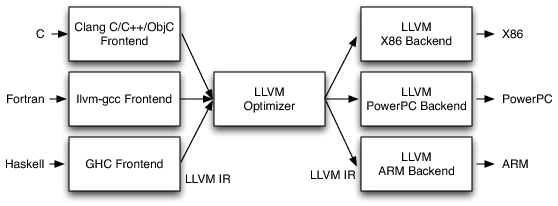
\includegraphics[width=\textwidth]{figures/llvm_arch.png}
    \caption{Diagram of LLVM compiler infrastructure's architecture. Reprinted from \cite{LattnerAOSA}}
    \label{fig:llvm_arch}
\end{figure}

Other compiler projects take a similar approach to their architecture. The GNU Compiler Collection uses several Intermediate Representations throughout the compilation process \cite{Novillo2004} - GENERIC, an abstract syntax tree representation; GIMPLE, a three-address-code representation; and a register transfer language - to simplify operations in different sections of the pipeline, and help modularize an otherwise monolithic architecture. Ongoing efforts \cite{GCCRearch} are being undertaken to further modularize this system into separate front-end, middle-end and back-end modules.
CompCert\cite{Leroy2009Compiler}, a formally verified compiler for the C programming language, also uses several intermediate representations to aid their goal of implementing and verifying each stage of the compilation process (see Figure ~\ref{fig:compcert_arch}).

\begin{figure}
    \centering
    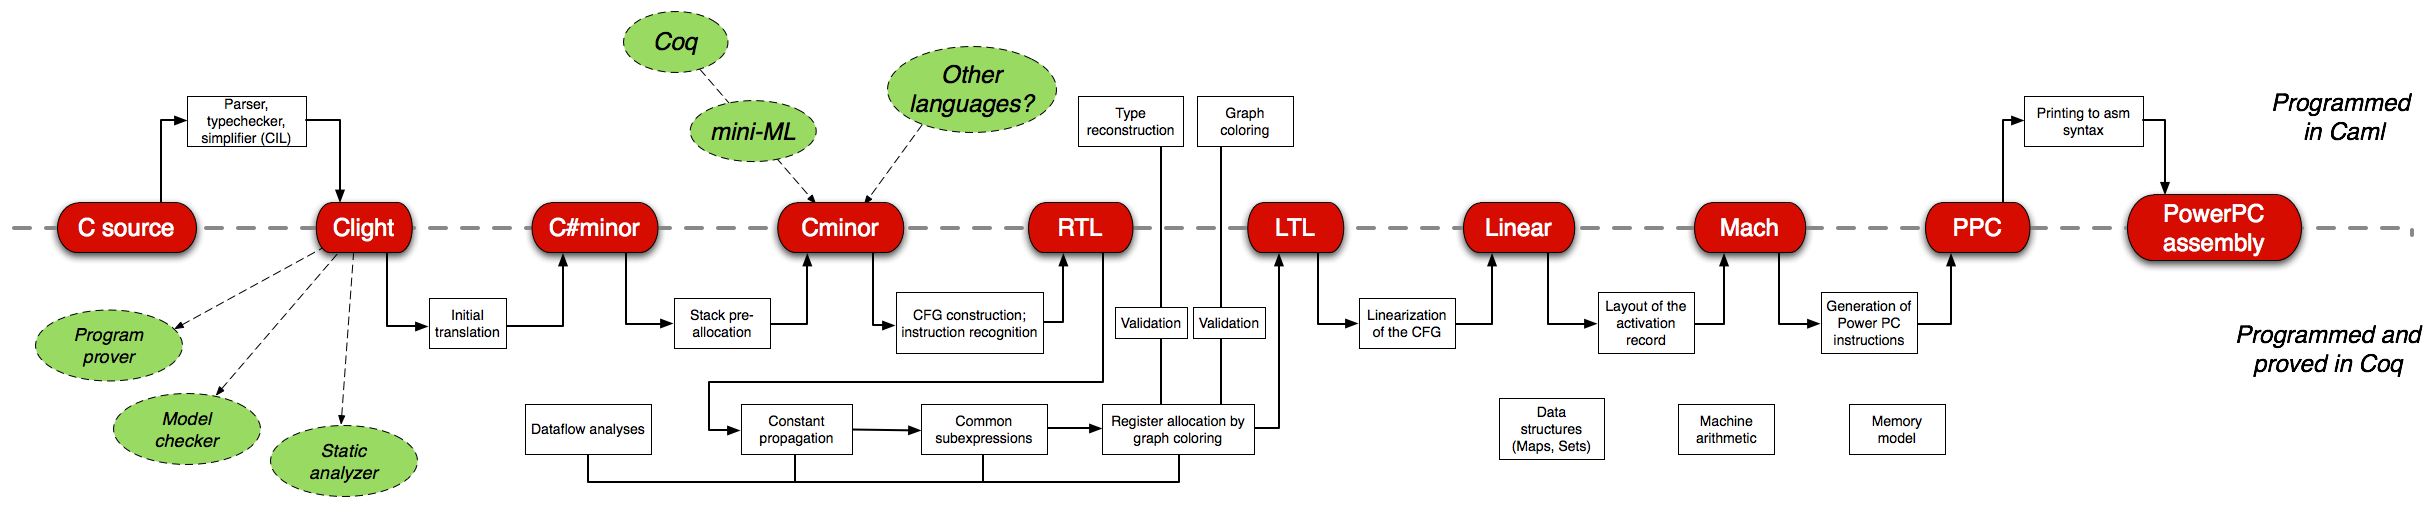
\includegraphics[width=\textwidth]{figures/compcert_arch.png}
    \caption{Diagram of CompCert's architecture. Reprinted from \cite{CompCertHome}}
    \label{fig:compcert_arch}
\end{figure}

\section{Optimization Techniques}

For the aims of our work, it proves useful to understand the kind of techniques that are commonly utilized to transform user-supplied codes into equivalent, yet more performant programs. This is done through analyzing the code and determining opportunities for transforming it into an optimized form, and performing those transformations, usually as a series of \textit{passes}, which yield a transformed version of the program.

We specifically wish to highlight two different aspects of the optimization process: the scope of the analyses, and the nature of the applied transformations.

\subsection{Scope of analysis for optimization}

Seeing as the first step of the optimization process is an analysis step, to determine which optimizations can be applied, we can distinguish optimizations by which scope the analysis is done.

The smallest scope is \textbf{local code analysis}. This analysis considers distinct instructions or small blocks of instructions. For example, let us consider the \textit{strength reduction} optimization. This optimization substitutes specific instances of complex instructions for equivalent but simpler, and therefore faster to execute, instructions. Consider the following two codes:

\begin{lstlisting}[language=C]
// prologue
// assume this variable exists and is set through an external interaction
int input_var;

// before strength reduction
int transformed_var = input_var * 4;

// after strength reduction
int transformed_var = input_var << 2;
\end{lstlisting}

The analysis is able to transform a multiplication by a power of two by an equivalent arithmetic shift instruction. Notice that, to perform this optimization, the analysis needs to just consider the one line of code, or a small block of instructions (load from memory, multiply with an immediate, store to memory). Therefore, it is \textit{local} in scope. In fact, this optimization can even be applied by linearly scanning the generated low-level code and replacing the instruction directly, in a process called \textit{peephole optimization}.

An intermediate scope at which analyses can be performed, and probably the most common one, is that of \textbf{global code analysis}\cite{Kildall1973}. This kind of analysis considers all visible code in a self-contained block, which usually corresponds to a function or procedure in the high-level language. Because such a scope might contain branching control and data-flow, stemming from the existence of loops and conditionals, these analyses rely on more advanced techniques, such as control and data-flow analysis\cite{Cytron1991}, logical induction of variables, etc, but in turn are able to deliver transformations that stem from the interaction between different blocks of instructions.

Some examples of this scope of analyses are:

\begin{itemize}
    \item Constant folding and propagation, or compile-time evaluation - this technique substitutes complex expressions whose arguments are only constants by the use of a single constant, that is yielded by performing the computation at the time of compilation.
    \item Common sub-expression elimination - this analysis detects expressions where a factor is repeatedly computed, and reworks the code to only compute it once, storing its value in a temporary variable to be reused.
    \item Loop unrolling - this analysis duplicates the body of a loop in the code, to perform fewer branches, which may improve instruction pipelining on the CPU.
    \item Dead code elimination - eliminates sections of the code which are unreachable, based on an analysis of the program's control flow.
    \item Some kinds of strength reduction, such as substituting the iterative computation of an arithmetic series by its direct computation, are only possible through global analyses, such as inductive variable analysis.
\end{itemize}

Even though this scope of analysis often suffices to perform many useful transformations, it carries the limitation that calls into other global scopes, such as calls to other functions, procedures, and units of compilation, are opaque, meaning that transformations which need information from several global scopes are impeded. To solve that issue, another scope of analysis is needed, \textbf{inter-procedural analysis}. On this scope, the interactions between different procedures are considered by analyses. Let us consider the following code as an example:

\begin{lstlisting}[language=C++]
template <type T>
class vector<T> {
    const T get(size_t i) const  {
        if (i < size) {
            return array[i];
        } else {
            throw Exception(/*...*/);
        }
    }

    size_t get_size() const {
        return size;
    }


    private:
    T* array;
    size_t size;
}

int main(void) {
    auto vec = new vector<int>();

    // initializing code here ...

    for (size_t i = 0; i < vec.get_size(); i++) {
        auto elem = vec.get(i);
        std::cout << elem * elem << '\n';
    }
}
\end{lstlisting}

In this code listing, we can intuit that there are several optimization opportunities that go unexploited unless we consider the interaction between both functions:

\begin{itemize}
    \item On line 26, a naïve call to the \textit{get\textunderscore{}size} function will involve multiple operations related to calling the function - saving to the stack a number of values whose registers might be overwritten, storing the parameters and the return instruction pointer in specific registers or stack positions, jumping to the subroutine, storing the return values in specific registers or stack positions, jumping back to the callee, restoring the values that were previously ejected from the registers, etc - even though the body of the function itself consists only of loading a number from a memory address. By using an inter-procedural analysis such as \textit{function inlining}, which duplicates the body of the called function inside the body of the caller, the compiler is able to remove such operations, yielding a simpler version of the code.
    \item While we can recognize that the loop header in line 26 and the branch in line 4 contain a duplicated condition check, simple global analysis in each procedure will not be able to detect such redundancy. However, an \textit{inter-procedural dead code elimination} analysis is able to do so, and remove the redundant check and associated unreachable code.
\end{itemize}

\subsection{Nature of transformations}

When considering which transformations can be applied in the context of optimizing codes, we distinguish the nature of the transformation, in relation to how it affects the performance of the code and the process of optimization itself.

Often, a transformation can itself be considered a \textbf{direct optimization}. The nature of these transformations is that they directly improve the performance of the transformed code. For example, strength reduction operations directly substitute computations for equivalent yet cheaper operations, directly improving the speed of the code. Likewise, constant propagation and folding allows computation to be shifted from run-time to compilation time, allowing expensive computations to be replaced by cheap loading of an immediate value.

On the other hand, some transformations might benefit the optimization process, regardless of their direct impact on the codes' performance. We term these \textbf{enabling transformations}. These transformations enable previously impossible optimizations, surfacing an emergent optimization property from the composition of different techniques\cite{Click1995}.

For example, function inlining may or may not impact positively the performance of the code\cite{Chen1993}, depending on the balance between the improved instruction pipelining, and the worsened program size, which may affect negatively the caching of the program's instructions. In any case, the extra information that the body of the inlined function provides may be instrumental in performing other analyses and transformations, such as dead code elimination, vectorization, or constant folding.

Another example of this phenomenon is constant folding and propagation. Besides directly reducing the amount of computation performed at run time, it may enable the compiler to prove that certain code paths are unreachable, aiding the process of dead code elimination.

Furthermore, some transformations, which are often called \textit{normalization} transformations, have the explicit goal of putting the analysed codes in a \textit{canonical form}, so that latter analyses have fewer edge cases to contend with, making the transformation code simpler and more maintainable. Examples of these include factoring complex computations into several temporary variables, or normalizing loop headers\cite{Gomes2021} e.g. so that they are always of the form \texttt{for (int i = 0; i < N; i++)}.

\section{Summary}

In this chapter, we have given an overview of important background concepts, for our work, namely by describing the three-stage architecture of modern optimizing compilers, and by categorizing the scope and nature of the analyses and transformations that they may perform on the programs they compile.
\chapter{Related Work}\label{chap:sota-lit}

To meet the challenges presented in Section ~\ref{sec:motivation}, several distinct approaches have been proposed and developed.

\section{Developments in IR-based optimization approaches}

\subsection{Mid-level Intermediate Representations}\label{sec:midlevel-ir}

As high-level languages have expanded their breadth to capture more semantic details, several compiler infrastructures have introduced their own IR between the high-level language, and AST, and the underlying optimizer, and its respective low-level IR.

These representations generally work on an intermediate level of abstraction, in which the set of syntactic constructs is restricted, and the semantic details of the language are encoded, as opposed to being eliminated in the process of lowering to a low-level IR.

Several of these approaches have been identified \cite{Lattner2021}:

\begin{itemize}
    \item The Rust compiler lowers the programs written in the language to their internal IR, MIR\cite{RustMirRfc}. This representation eliminates several syntax constructs to facilitate several analyses, such as liveness, death and reachibility checking, borrow checking (which implements Rust's static guarantees of memory safety), and guiding translation to the lower-level LLVM-IR.
    \item The Swift compiler lowers the programs to the Swift Intermediate Language (SIL) \cite{SwiftSIL}, which they use to provide the following analyses: "A set of guaranteed high-level optimizations [...]. Diagnostic dataflow analysis passes that enforce Swift language requirements [...]. High-level optimization passes [...]. A stable distribution format that can be used to distribute 'fragile' inlineable or generic code with Swift library modules, to be optimized into client binaries."
    \item The Julia compiler lowers the programs to a SSA-form representation \cite{JuliaIR} after performing macro inlining and other syntax simplification tasks, in order to perform middle-end optimization tasks.
\end{itemize}

While the intermediate level of abstraction might be appropriate for some optimizations, this approach is limited by several factors.

Firstly, it still ties the optimization work to a single compiler implementation: whereas these languages have had their effort mostly concentrated on a single implementation (Swift compiler, \textit{rustc}, and the Julia compiler) and so are able to mitigate this disadvantage, other source languages, such as C and C++, have multiple compiler implementations, where this approach suffers from a fragmentation of effort.

Moreover, this approach continues to necessitate a lowering of the level of abstraction, which might impede optimization efforts that depend on high-level details of the programming language. This effect is exacerbated when considering the use cases of finding optimizations for codes that make use of eDSLs or libraries \cite{Zangerl2018}.

\subsection{MLIR: Declarative approach to defining and optimizing a Multi-Level Intermediate Representation}

Another recent contribution in this space is MLIR \cite{Lattner2021}. This extension of the LLVM representation aims to deal with several deficiencies of that system's approach to compilation, namely shortcomings in dealing with heterogeneous targets and non-scalar data.

To that end, it formalizes a system of intermediate representation with the following characteristics:

\begin{itemize}
    \item Ability to capture multiple levels of abstraction through the use of nested blocks of operations, and the use of attributes to capture semantic details of tagged code regions.
    \item Separation of concerns between different translation passes through the definition of dialects, static traits and dynamic interfaces.
    \item Ability to define schemas for non-scalar data.
    \item Declarative approach to defining code transformations, including the ability to progressively and partially lower the abstraction level of code regions.
\end{itemize}

A practical example of this approach is the recently proposed Clang Intermediate Representation \cite{CirRfc} (CIR). This representation leverages MLIR's ability to define dialects and transformations within and between them to provide an intermediate language that does not necessarily rely on the syntactic constructs of the C and C++ languages, but allows important semantic concepts from these languages to be abstractly represented and reasoned about in analyses, before being morphed into other, and lower-level, IR dialects.

While this approach might prove valuable in its stated goal of generalizing and driving a wide goal of compiler projects, the generic nature of the representation may worsen the ergonomics of developing code transformations. In particular, the transformation implementer must learn the semantics of the IR representation, which is constructed to support the semantics of the language but not derived from it, and how to perform transformations on it. In the case of MLIR, the implementer must, depending on the specifics of their transformation, implement the transformation in terms of an external DSL and Python bindings, or even may need to write out their transformation imperatively, using a C++ template-based system.

In comparison, using source-to-source compilation allows us to provide a simpler development experience to users. By relying on the structure and semantics of widely supported high-level languages (C and C++), we are able to support a wide range of targets and assure the users that if they are able to implement the transformation on high-level code, they will be able to automate it. By relying on source-code normalization and simplification passes, we are able to provide a representation that is derived from the high-level language by subtraction, which can more immediately be understood (it is "just a simple C/C++"). Not only that, by providing an compiler interface embedded on, or embedding, an extremely popular and easy-to-use language such as Javascript, we are able to provide the optimization developers-to-be with a more ergonomic experience.

\section{C Intermediate Language: Source-to-Source normalization of C code}

Another work that is particularly relevant for this dissertation is the C Intermediate Language \cite{Necula2002}. This project is similar to, and can be in some ways considered to be a precursor of, our work, as it similarly recognizes that the C language has a wealth of complex constructs hampering a straightforward analysis process of source programs.

To tackle this issue, it constructs a high-level representation that preserves most semantic aspects of the C source code, but simplifies several aspects of the language, including removing redundant constructs and syntactic sugar, making implicit casts explicit, and separating value evaluation, side-effect creation, and control-flow changes. It also incorporates a Control Flow Graph into the representation to make analyses relying on it simpler. After converting to this representation, it applies any transformations that the user has specified, using an embedded DSL in OCaml, and outputs the transformed program in C.

As close as this approach may be to our work, there are still some different trade-offs between this approach and ours:

\begin{itemize}
    \item This approach still works by constructing a new representation that, while mapping closely to the source language, still is separate from it. While this allows for a significant transfer of domain knowledge compared to other IR-based approaches, it still is not as close to the source language as we desired. In comparison, our AST-based approach, which only subtracts elements that are deemed too complex, keeps a more faithful representation of the original program.
    \item The language proposed by the authors eliminate some features, such as some kind of syntactic sugars (\verb|->|) or scoped variable declarations, that we consider to be useful enough and simple enough that they do not hamper the analysis of the language, while departing from the original program.
    \item The front-end parser for the language is rather limited, only supporting ANSI C with some GNU and MSVC extensions. While this is understandable when considering the age of the tool, it stands in contrast with Clava, which is able to use Clang's frontend tooling to support codes written not only in C, but also C++ and OpenCL, evolving to support more recent features of the language as Clang evolves to support them too.
    \item When implementing further transformations, CIL requires them to be written using a limited interface based on OCaml and using only a visitor pattern. In contrast, the LARA environment that Clava uses allows full access, including imperative modification if needed, to the program's AST, using a widely-used host language (Javascript).
    \item While CIL does preliminary analysis to present a unified CFG and AST representation of the program, this needlessly complicates reasoning about program when such analysis is not required. In the Clava standard library, we implement normalization and control-flow analysis separately, improving separation of concerns between these two tasks.
\end{itemize}

\section{C--: Reduced C-language Subset as Compilation Target}

Another set of authors that historically proposed the use of a reduced subset of C as a language to be used by compilers is Peyton Jones, Ramsey, and Reig, with C-- \cite{Jones1999}.

In their work, the authors identify several limitations encountered by using C as a portable assembly language to be targeted by compiler front-ends for other abstract programming languages. Specifically, they mention the lack of support of continuations, multiple return in registers, control of the stack framing and calling conventions, among other deficiencies as severely limiting to implementing functional languages like Haskell, ML, or Scheme.

To solve this issue, they propose a language that at first sight looks like a simplified version of C, but is not a proper subset. They define abstractions to control a number of lower-level behaviors, such as precise control over static data layout, and stack-less jumps to implement continuations or perform tail call elimination.

While there is stand-alone value in this approach for its purported use case of providing a portable target to implement high-level languages, though a fair comparison with more recent contributions in IRs \cite{Lattner2004} is warranted, this approach does not meet our particular use case.

With our contribution, our goal is to support an optimization use case for compiler-independent analysis and transformation of C and C++ programs, not programs in other languages. That means that it is more ergonomic to provide a representation that captures a proper subset of our source languages, and we do not feel the need to break the confines of the C and C++ languages as they are specified.

\section{Formally-verified optimization techniques for certified compilers}

In the context of certified compiler implementation, several recent contributions have aimed to implement formally-verified optimizations for the CompCert project:

\begin{itemize}
    \item Tristan and Leroy, 2009 \cite{Tristan2009} implement and formally verify a Lazy Code Motion optimization pass.
    \item Barthe et al, 2014 \cite{Barthe2014} contribute a formally-verified middle-end that adopts an SSA-form intermediate representation, which simplifies the implementation of further optimizations.
\end{itemize}

These two contributions have in common the use of a combined technique for implementing verified compilers. Specifically, the respective authors follow a process where they implement the optimization pass using an unverified algorithm, for performance purposes, and introduce a subsequent verification pass where a formally-verified validator program checks the correctness of the transformation.

Another contribution in this space is a formally-verified implementation of a global common sub-expression elimination and loop-invariant code motion pass \cite{Monniaux2021}.

These contributions prove that, with enough effort, it might be possible to formally verify and implement a large breadth of optimization techniques, but several concerns remain unaddressed:

\begin{itemize}
    \item The optimization work is still tied to a specific compiler. This aspect is exacerbated by the consideration that other compilers' models might not be formally specified or validated to the same extent, and that the presence of differing abstractions between compilers will now entail not only the need to adapt the implementation, but also the validation step.
    \item Although we consider these contributions a good first step in proving that it is possible for certified compilers to be enhanced in their optimization abilities, there are other reasons that might impede their modification by users and researchers, such as their being proprietary or other impeding circumstances.
    \item In some cases, namely during prototyping work, it might be desirable to work with a single, high-level abstraction, whereas the process of verification necessitates multiple, more detailed formal constructs.
\end{itemize}

For this reason, we consider that the use of source-to-source compilation, followed by the use of a certified compiler for the final compilation step, might be a good middle-of-the-road alternative to provide a degree of safety and simultaneously allow for research into new optimization techniques.

\section{Summary}

In this chapter we have given an overview of recent related contributions to our work. We found that there have been efforts in providing more flexibility to IR-based approaches and in formally-verifying optimization passes for certified compilers.

We reached the conclusion that there is space to push further with a source-to-source compilation approach to analysis and transformation, which we detail in Chapter ~\ref{chap:gen_approach}.
\chapter{Automatic C/C++ source-code normalization and optimization} \label{chap:stmt}

\section{Problem Statement}

There is room for improvement in the ergonomics of developing optimization techniques for C and C++ code. Merely doing so through the extension of existing compilers presents challenges in portability and maintainability and may not be feasible in certain cases.

Is source-to-source compilation a feasible technique for implementing optimizing and normalizing code transformations? Can this technique provide more legible, composable transformations as IR-based approaches, while being similarly effective?

\section{Proposed Solution}

We will identify a set of normalizing or optimizing code transformations to be implemented using source-to-source compilation techniques.

These transformations will be implemented as a library for the Clava source-to-source compiler.

\section{Validation and Expected Results}

The results of our work will need to be validated according to the following criteria:

\begin{itemize}
    \item Feasibility of implementation: for each identified transformation, we will evaluate whether it was feasible to successfully implement it using a source-to-source compilation approach, and compare it to its feasibility using traditional techniques.
    \item Maintainability of implementation: for each identified and implemented transformation, we will evaluate, in subjective terms, whether the implementation is made simpler and more maintainable by the use of source-to-source compilation.
    \item For optimizing transformations, effectiveness of the transformation: representative programs will be compiled with and without the transformation, under different compiler configurations, and benchmarked to measure the performance effects of the optimizations.
    \item For normalizing transformations, composability of the transformation: we will subjectively evaluate the enabling effects of these transformations, by discovering which further optimizations are enabled by their application.
\end{itemize}

We expect that the transformations that we implement are done so in a clearer way than with other approaches, especially those optimizations that rely on higher-level semantics of the source language.

Furthermore, we expect that the optimizations that we implement will yield positive performance effects, especially when using less optimizing compilers, such as those compilers configured with -O0 and -O1 flags, or less developed compilers.

Finally, we expect that the implementation of normalizing transformations will enable further optimizations to be implemented in the future.

All in all, we expect that \textbf{our main contribution will be a proof of concept for the possibility of developing generalized and automatic optimizations with source-to-source compilers}.

\section{Work Proposal}

We propose the following schedule for our work:

\begin{itemize}
    \item In the past three months, from December 2021 to February 2021, we have identified the problem that we wish to tackle, as well as our proposed approach to tackle it. Initial research into related work and literature has been carried out.
    \item In the initial phase of our research, we will identify the set of transformations that we wish to implement, and extend our research into related work.
    \item We will then implement and measure the results of these transformations, using the Clava compiler.
    \item In the final phase of our work, we will validate and evaluate the results of our implementation, and draw the respective conclusions from that evaluation process.
\end{itemize}

Figure ~\ref{fig:gantt} shows a Gantt chart of the intended work schedule.

\begin{sidewaysfigure}
    \centering
    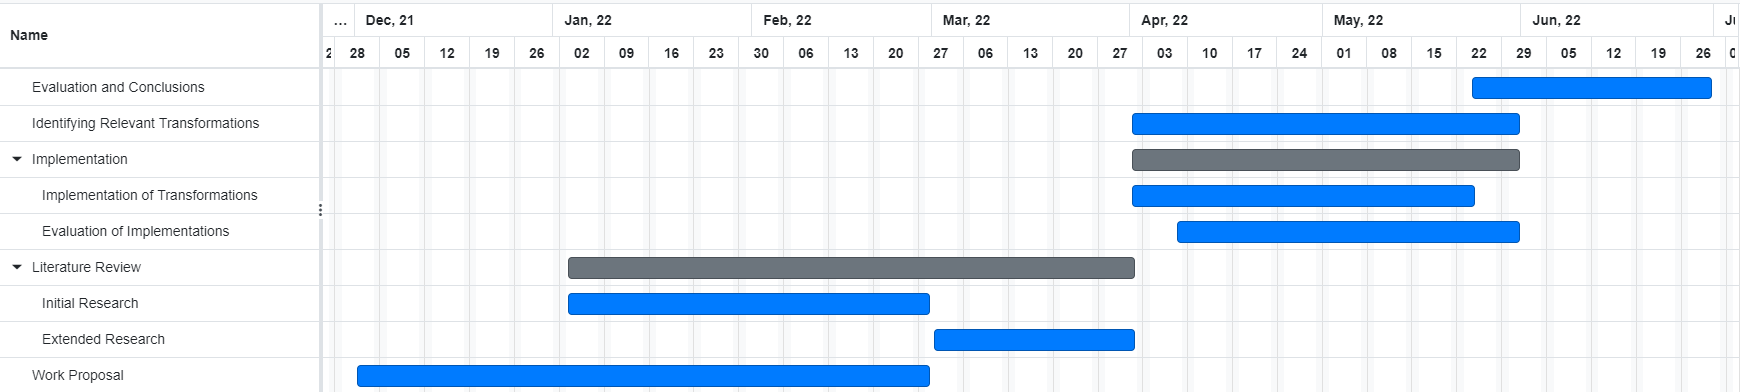
\includegraphics[width=\textwidth]{figures/gantt.png}
    \caption{Gantt chart of intended work schedule}
    \label{fig:gantt}
\end{sidewaysfigure}
\chapter{Conclusions} \label{chap:concl}

\section*{}

In this work, we have identified an ergonomics problem affecting the research and implementation of source-code transformations, especially those that aim to optimize non-functional aspects of compiled programs through extensions to existing compilers.

We hypothesize that this problem is mainly caused by a mismatch between the level of semantics at which compilers operate and at which the source code is expressed, and the operational challenges of extending and maintaining an extension or alternate distribution of existing compilers.

Moreover, we have given an overview of important background concepts and of related contributions in this area of work. Finally, we have proposed a solution to this problem, making use of source-to-source compilation as the technique to drive it, and identified the key validation and evaluation criteria for it.

Throughout the next phases of this work, we will carry out more extensive research into related work, implement our solution, and evaluate it, according to the criteria that have been identified.
 

%% comment next 2 commands if numbered appendices are not used
%\appendix
%\include{appendix1}

%%----------------------------------------
%% Final materials
%%----------------------------------------

%% Bibliography
%% Comment the next command if BibTeX file not used
%% bibliography is in ``myrefs.bib''
\PrintBib{myrefs}

%% Index
%% Uncomment next command if index is required
%% don't forget to run ``makeindex pdis'' command
%\PrintIndex

\end{document}
